% !TeX root = ../../main.tex

\section{Business scenarios}

\begin{table}[H]
\centering
\caption{Scenario analysis for different cases}
\label{scenario_analysis}
\begin{tabular}{l|llll}
\rowcolor[HTML]{D2F3FA} 
                      & \multicolumn{4}{c}{\cellcolor[HTML]{D2F3FA}\textbf{Scenarios}}                                                          \\
\rowcolor[HTML]{D2F3FA} 
\textbf{Parameter}    & \textit{\textbf{Best case}} & \textit{\textbf{Base case}} & \textit{\textbf{Worst case}} & \textit{\textbf{COVID case}} \\
WACC                  & -30\%                       & -                          & 30\%                         & -                            \\
CAPEX                 & -30\%                       & -                          & 30\%                         & -                            \\
Price of product      & 30\%                        & -                          & -30\%                        & -                            \\
Production delay      & No delay                    & No delay                   & 3 year delay                 & 3 year delay                 \\
Operational days      & -                           & -                          & -                            & -40\%                        \\
Cost of raw materials & -                           & -                          & -                            & -40\%                        \\
Interest rate         & -                           & -                          & -                            & -40\%                       
\end{tabular}
\end{table}


Four scenarios were analysed to determine the combined effect of the parameters tested in Section XX. Table XX summarises the fluctuations made in each scenario. The best- and worst-case scenarios were based off the most extreme variations of each parameter in the sensitivity analysis. 

\begin{wrapfigure}{r}{8cm}
\caption{Discounted Cash Flows profile in different cases}
\label{DCF_scenario}
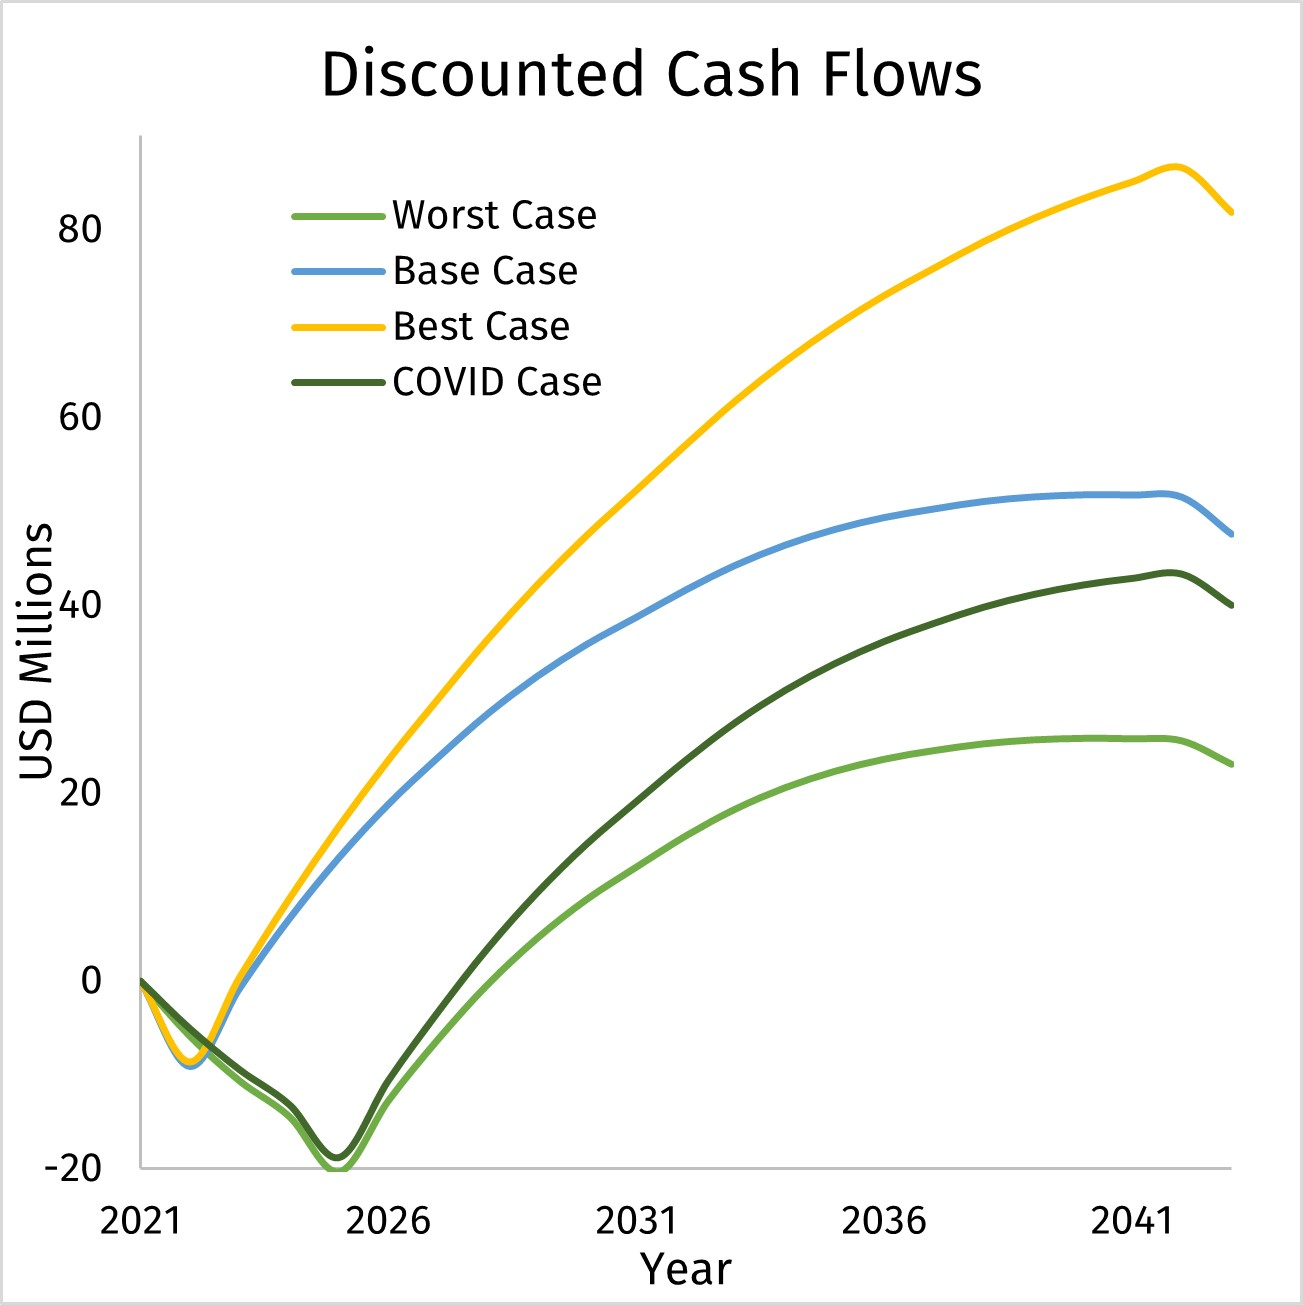
\includegraphics[\width=0.2\linewidth]{chapters/6-economics/figures/DCF.jpg}
\end{wrapfigure}

One particular scenario was related to a situation where COVID-19 resurfaced in Nanjing, China, and strong restriction measures were in place till 2026. The number of operational days per year was expected to drop by 40\% based on lockdown measures from the initial outbreak of coronavirus in 2020. A 40\% decrease in the cost of raw materials was also modelled into the scenario, based on the fall in toluene prices between January and April 2020. Similarly, a 40\% decrease in Nitroma’s interest rate was applied, based off the drop in the Chinese interest rate between January and April 2020. Furthermore, a 3-year delay in production was expected due to reduced labour availability. The price of Nitroma’s products was not expected to change considerably, as discussed in Section XX. It should be noted that the coronavirus conditions were only applied until 2026, after which the base case conditions were restored in the financial model.

Figure XX shows Nitroma’s discounted cash flows till 2043 for each tested scenario. Across all tested scenarios, the minimum ending cash balance was \$23.1 million and the longest payback period was 10.3 years. These results show the robustness of this project and should enhance the confidence of the shareholders.
